\documentclass[border=10pt]{standalone}

%Drawing
\usepackage{tikz}

%Tikz Library
\usetikzlibrary{angles, quotes, intersections}

%Notation
\usepackage{physics}
\usepackage{bm}

\begin{document}
	
	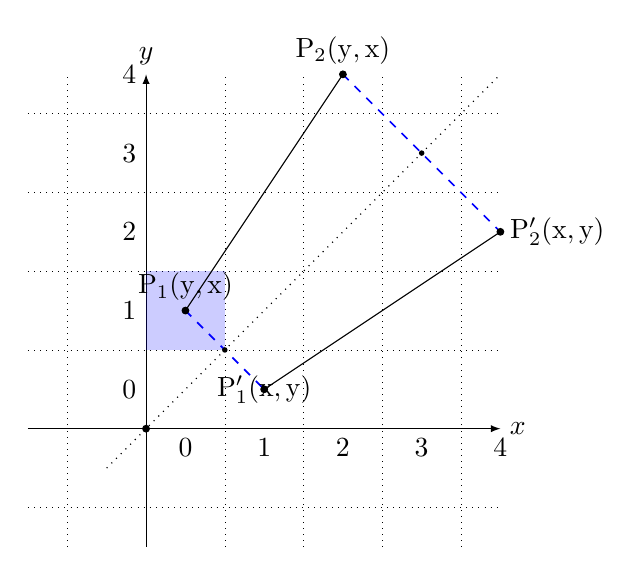
\begin{tikzpicture}
	
%Axis		
\draw[very thin,-latex] (-1.5,0) -- (4.5,0) node [right] {$x$};
\draw[very thin,-latex] (0,-1.5) -- (0,4.5) node [above] {$y$};

%Octants	
%\draw[dotted, thin] (-0.5,-0.5) -- (4.5,4.5);


%Grid
\draw[very thin, dotted] (-1.5,-1.5) grid (4.5,4.5);
\foreach \i in {0, 1,...,4}
{
	\node[below] at (\i+0.5,0) {\i};	
	\node[left] at (0,\i+0.5) {\i};	
}


\foreach \x/\y in {0.5/1.5}
{
	\fill[blue, opacity=0.2] (\x-0.5,\y-0.5) rectangle (\x+0.5,\y+0.5);  
}

	
%%%%%%%%%%%%%%%%%%	
%Coordinates		

\coordinate (O) at (0,0);
				
\coordinate (start) at (0.5,1.5);
\coordinate (start') at (1.5,0.5);


\coordinate (end) at (2.5,4.5);
\coordinate (end') at (4.5,2.5);

%Lines	
\draw[black,thin] (start) -- (end);
\draw[black,thin] (start') -- (end');

\draw[name path=octant, dotted, thin] (-0.5,-0.5) -- (4.5,4.5);	

\draw[name path=starts, blue, dashed, semithick] (start) -- (start');
\draw[name path=ends, blue, dashed, semithick] (end) -- (end');




\path [name intersections={of=starts and octant, by=start-int}];
\path [name intersections={of=ends and octant, by=end-int}];
\fill[black] (start-int) circle (1pt) ;
\fill[black] (end-int) circle (1pt) ;
				


% Points			
\draw[fill=black, draw=black] (O) circle (1.2pt);
%\draw[fill=black, draw=black] (3,3) circle (1.5pt);


% end of blue lines	

\draw[fill=black, draw=black] (start) circle (1.2pt);
\draw[fill=black, draw=black] (start') circle (1.2pt);
\draw[fill=black, draw=black] (end) circle (1.2pt);
\draw[fill=black, draw=black] (end') circle (1.2pt);



% Nodes

\node[above] at (start) {$\mathrm{P_1(y,x)}$};
\node[] at (start') {$\mathrm{P_1'(x,y)}$};

\node[above] at (end) {$\mathrm{P_2(y,x)}$};
\node[right] at (end') {$\mathrm{P_2'(x,y)}$};




\end{tikzpicture}
	
\end{document}